\documentclass[tikz,border=2pt]{standalone}
\usepackage{amsmath}
\usepackage{pgfplots}
\pgfplotsset{compat=1.18}
\usetikzlibrary{arrows.meta}
\begin{document}
% Exercise 7.2 data, nonbasic x_2 with reduced cost 2 and y^*=(2,1,0): changing a_{i2} by delta gives the
% new reduced cost 2+delta*y_i^*, a line of slope y_i^*; it crosses 0 at delta=-1 (a_{12}=0) and delta=-2
% (a_{22}=-1), and never for a_{32} (y_3^*=0). Below 0 the basis is no longer optimal.
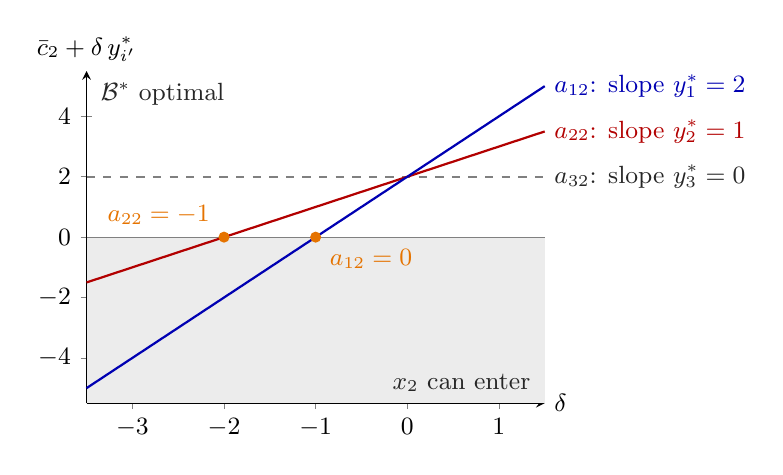
\begin{tikzpicture}[font=\small, >={Latex[length=2mm]}]
  \begin{axis}[
    axis lines=left, xmin=-3.5, xmax=1.5, ymin=-5.5, ymax=5.5,
    xtick={-3,-2,-1,0,1}, ytick={-4,-2,0,2,4},
    xlabel={$\delta$}, ylabel={$\bar{c}_2+\delta\,y_{i'}^*$},
    xlabel style={at={(axis description cs:1,0)}, anchor=west},
    ylabel style={rotate=-90, at={(axis description cs:0,1)}, anchor=south},
    width=7.4cm, height=5.8cm, clip=false
    ]
    \fill[gray!15] (axis cs:-3.5,-5.5) rectangle (axis cs:1.5,0);
    \draw[gray, thin] (axis cs:-3.5,0) -- (axis cs:1.5,0);
    \node[gray!30!black, anchor=south east] at (axis cs:1.45,-5.45) {$x_2$ can enter};
    \node[gray!30!black, anchor=north west] at (axis cs:-3.45,5.45) {$\mathcal{B}^*$ optimal};
    \addplot[gray, thick, dashed, domain=-3.5:1.5, samples=2] {2};
    \addplot[red!70!black, thick, domain=-3.5:1.5, samples=2] {2+x};
    \addplot[blue!70!black, thick, domain=-3.5:1.5, samples=2] {2+2*x};
    \node[blue!70!black, anchor=west] at (axis cs:1.5,5) {$a_{12}$: slope $y_1^*=2$};
    \node[red!70!black, anchor=west] at (axis cs:1.5,3.5) {$a_{22}$: slope $y_2^*=1$};
    \node[gray!30!black, anchor=west] at (axis cs:1.5,2) {$a_{32}$: slope $y_3^*=0$};
    \fill[orange!90!black] (axis cs:-1,0) circle (2pt) (axis cs:-2,0) circle (2pt);
    \node[orange!90!black, anchor=north west] at (axis cs:-0.95,-0.1) {$a_{12}=0$};
    \node[orange!90!black, anchor=south east] at (axis cs:-2.05,0.1) {$a_{22}=-1$};
  \end{axis}
\end{tikzpicture}
\end{document}
